%=============================================================================
% FIT (Frontiers of Information Technology) — IEEE two-column conference format
%
% FIT requirements confirmed from https://fit.edu.pk/submission-guidelines.aspx
%   - two-column IEEE conference format
%   - PDF, submitted via EasyChair
%   - must not be under consideration elsewhere
%
% PAGE BUDGET: 7-9 pages including references. Currently 9 — at the ceiling,
% so anything added must displace something.
%
% This is the FINDINGS paper (evaluation, leakage, transfer). The governance
% architecture — arbitration over a harm matrix, the answerability gate,
% provenance, injection defence — is the companion paper, preserved in
% main_system_paper.tex. Do not reintroduce architecture here without cutting.
%
% Build:  powershell -File compile.ps1   (pdflatex, bibtex, pdflatex, pdflatex)
% It prints the page count. Check it EVERY build; the count includes references.
%=============================================================================
\documentclass[conference]{IEEEtran}
\IEEEoverridecommandlockouts

\usepackage{cite}
\usepackage{amsmath,amssymb}
\usepackage{algorithmic}
\usepackage{graphicx}
\usepackage{textcomp}
\usepackage{xcolor}
\usepackage{booktabs}
\usepackage{url}
\usepackage{microtype}

\setlength{\floatsep}{3pt plus 1pt minus 1pt}
\setlength{\textfloatsep}{4pt plus 1pt minus 1pt}
\setlength{\intextsep}{3pt plus 1pt minus 1pt}
\setlength{\abovecaptionskip}{2pt}
\setlength{\belowcaptionskip}{1pt}

% Draft-only marker. DELETE this macro and every use of it before submitting.
\newcommand{\TODO}[1]{\textcolor{red}{\textbf{[TODO: #1]}}}

\begin{document}

\title{In-Distribution Gains Do Not Transfer: Leakage-Free Evaluation of
Retrieval Interventions for Low-Resource Legal Question Answering}

\author{\IEEEauthorblockN{Muhammad Usama$^{1}$ and Muhammad Amir Zarmaan Ullah Khan$^{2}$}
\IEEEauthorblockA{\textit{$^{1,2}$Department of Computer Science, COMSATS University Islamabad, Pakistan}\\
Email: \href{mailto:muhammadusamahoyrr@gmail.com}{\underline{muhammadusamahoyrr@gmail.com}}, \href{mailto:kzari898@gmail.com}{\underline{kzari898@gmail.com}}}}

\maketitle

%, , , , , , , , , , , , , , , , , , , , , , , , , --
\begin{abstract}
Retrieval interventions for legal question answering are almost always reported
as a single number on a single evaluation set, and that number is almost always
measured on questions drawn from the same distribution the system was tuned on.
We report what happens when it is not. Fine-tuning a multilingual retriever on
$4{,}692$ verified citation pairs for Pakistani law gains $+26.5$ Hit@1 on
held-out questions from its own generator and $+2.4$ when the question style
changes. A second model, trained on a tenth as much data from a different source,
initially shows a $+16.5$ in-distribution gain, but target leakage invalidates that
comparison; on clean out-of-distribution evaluation it changes by $-0.3$. Sorting every retrieval intervention we measured by whether its effect
survived a change of question style produces a clean split: those encoding legal
or document structure transferred, those learning question phrasing did not, including
a general-purpose cross-encoder that moved the correct statute from rank~3 to
rank~10 where a deterministic statutory-scope rule placed it first in under a
millisecond. We further report three evaluation defects---an index containing its
own test answers, a systematically wrong gold-label join, and target leakage between train and test---each of which inflated or distorted a headline number until it was
checked, and each time the flattering version was the wrong one; none was
visible in the metrics, and in each case the correction removed a result we had
already believed. Throughout, the measurement protocol determined the
conclusions more than any technique did.
\end{abstract}

\begin{IEEEkeywords}
legal informatics, retrieval-augmented generation, retrieval evaluation,
distribution shift, data contamination, low-resource NLP, code-switching, Urdu
\end{IEEEkeywords}

%, , , , , , , , , , , , , , , , , , , , , , , , , --
\section{Introduction}
Access to legal information is unevenly distributed. In Pakistan, where
legal counsel is scarce outside major urban centres and court backlogs leave
disputes unresolved for years, a litigant who cannot afford counsel is often
unable to establish even the threshold facts of their own position: which statute
governs, which forum has jurisdiction, what a filing will cost, or whether a
limitation period has already expired.

Retrieval-augmented generation~\cite{lewis2020rag} is the standard response, and
legal question answering is now an active application
area~\cite{chalkidis2020legalbert,guha2023legalbench}. Applying it to Pakistan
is not a matter of swapping the corpus. Queries arrive in English, in Urdu
script, and most commonly in Roman Urdu, the transliterated register used in
everyday digital communication; the applicable law combines codified statute
with Islamic personal law and varies by province; and users routinely import
Indian statutory terminology, asking about the Indian Penal Code when the
Pakistan Penal Code governs. Each is a retrieval problem before a generation
problem, and none has an established benchmark.

\textbf{Reproducibility.} All evaluation code, corpus ingestion manifests,
contamination detection scripts, and fine-tuning configurations are publicly
available to enable independent auditability.

That absence is the subject of this paper. When no independent evaluation set
exists, a system's developers build one, tune against it, and report the
resulting number, and the literature offers little guidance on how much such
a number is worth. We set out to improve retrieval for this jurisdiction and
measured each intervention twice: once on questions from the distribution it was
developed against, and once on questions written by a different generator for a
different purpose. The gap between those two measurements turned out to be
larger than the gap between any two techniques we tried.

We report it as a negative result with a positive structure. Interventions
divide by \emph{what they encode}: those encoding a property of the law or the
documents survived the change of question style, while those learning a mapping
from question phrasing to passage did not, however large their in-distribution
gain. The same division predicts which of our corpus repairs held.

\textbf{Scope of claims.} Several results below are defects we found in our own
system, reported as findings rather than apology: each was invisible to the
metric meant to catch it, and these failure modes are not specific to a single
model configuration. What we do \emph{not} claim is equally definite: no
end-to-end improvement in answer correctness, and no Pakistan-wide coverage.
Section~\ref{sec:threats} states each limit and what it bears on.

The system that produced these measurements is described only as far as the
results require (Section~\ref{sec:setup}); its architecture is reported
separately. Our contributions are:

\begin{itemize}
\item \textbf{A transfer measurement of retrieval fine-tuning}, over two models
trained independently at a tenfold difference in scale, with an account of why
that predicts which interventions transfer
(Sections~\ref{sec:finetune},~\ref{sec:whynot}).
\item \textbf{Three contaminations and how each was found}: a leaking index, a
systematically wrong gold-label join, and target leakage between test and
training, none visible in the metrics (Section~\ref{sec:leakage}).
\item \textbf{Verified citation supervision} for a jurisdiction with no
query/passage training data, built from citations because a citation is
checkable (Section~\ref{sec:citationdata}).
\end{itemize}

\section{Related Work}
\textbf{Legal NLP and retrieval-augmented generation.}
Domain-adapted encoders such as LEGAL-BERT~\cite{chalkidis2020legalbert}
established that legal text benefits from in-domain pretraining, and
LegalBench~\cite{guha2023legalbench} benchmarks legal reasoning in large
language models. Retrieval augmentation~\cite{lewis2020rag} over dense
passage retrieval~\cite{karpukhin2020dpr} is the standard architecture for
grounding answers in sources, with Self-RAG~\cite{asai2024selfrag} adding
self-reflection over retrieval quality. This line of work targets English
common-law or EU material almost exclusively, and reports in-domain evaluation
on benchmarks it did not construct, a luxury this jurisdiction does not
afford.

\textbf{Low-resource and hybrid retrieval.}
Multilingual dense encoders~\cite{wang2024multilinguale5} make a single index
viable across scripts, and hybrid lexical--dense retrieval with rank
fusion~\cite{robertson2009bm25,cormack2009rrf} remains strong where exact
terminology matters, as it does for statute references. Neither line reports
what fusion does to a dense channel fine-tuned on the domain, which
Section~\ref{sec:hybrid} measures.

\textbf{Generalisation and contamination in evaluation.}
That a retriever's gain may not survive a change of domain is established for
English: BEIR~\cite{thakur2021beir} evaluates retrievers zero-shot across
eighteen datasets and MTEB~\cite{muennighoff2023mteb} extends the idea to
embedding models generally, both finding in-domain strength a poor predictor of
out-of-domain strength. Neither has an analogue for a low-resource jurisdiction,
where the practical difficulty is that a developer must build the only
evaluation set that exists. Contamination is likewise recognised as a systematic
threat to reported results~\cite{magar2022contamination,sainz2023contamination},
though that literature concentrates on pretraining corpora absorbing benchmark
text; we report the retrieval-specific case, in which the \emph{index} is itself
a system component and can leak (Section~\ref{sec:leakage}).

What none of these lines reports, and what we report here, is whether a
retrieval intervention's measured gain survives a change in who wrote the
questions.

%, , , , , , , , , , , , , , , , , , , , , , , , , --
\section{Experimental Setup}
\label{sec:setup}

\subsection{Corpus and Retrieval}
\label{sec:retrieval}
The statute corpus is drawn from a public collection of 969 Pakistani legal
documents~\cite{paklaws}, itself converted from Ministry of Law and Justice
publications and distributed under ODC-BY; we segment it by section and
partition it into four collections by legal domain (civil, criminal, family,
constitutional). It is supplemented with instruments fetched directly from the
official consolidated legislation service~\cite{pakistancode}, including the
Code of Civil Procedure 1908 and twenty family-law statutes that the public
collection omitted. The constitutional collection holds article text
authenticated against the National Assembly publication; a bilingual
English--Urdu constitutional question--answer set~\cite{legaluqa} supplies
evaluation questions only and is \emph{not} indexed, for reasons
Section~\ref{sec:leakage} reports. A separate corpus of reported judgments
from six courts supports case-law retrieval. Figure~\ref{fig:corpus} reports the
indexed chunk counts. The sources are government publications under an
attribution licence, given here and in the released ingestion code.

\begin{figure}[t]
\centering
\vspace{-3mm}
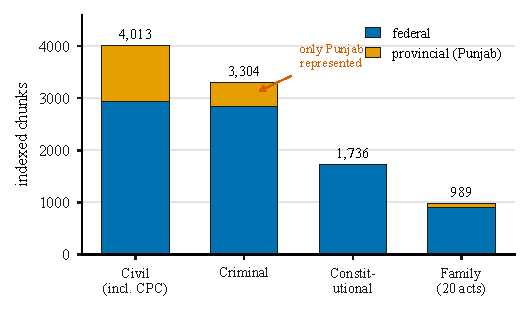
\includegraphics[width=0.81\columnwidth]{figures/fig1_corpus.pdf}
\vspace{-2mm}
\caption{Indexed statutory corpus by collection and legislative tier, with a
separately indexed judgment corpus of $7{,}529$ chunks from six courts not
shown. Devolved provincial coverage is Punjab-only; constitutional law is inherently federal.}
\label{fig:corpus}
\vspace{-3mm}
\end{figure}

Retrieval is hybrid. A BM25 index and a dense index over
\texttt{multilingual-e5-base} embeddings are combined by weighted ensemble with
weights $0.6$ and $0.4$ respectively, the lexical channel weighted higher
because exact statute and section references carry disproportionate signal in
this domain. Dense retrieval applies the asymmetric \texttt{query:}/
\texttt{passage:} prefixes the model expects. Both channels are filtered so that
a query for a given province retrieves only that province's provisions or
federal ones: the dense channel by metadata predicate, the lexical channel by
post-retrieval filter, since BM25 admits no index-time constraint.

That filter is a mechanism, not a coverage claim: of $10{,}042$ statutory
chunks, $1{,}608$ are provincial and all of them are Punjab
(Figure~\ref{fig:corpus}), so a query from any other province is served from
federal law alone. Since tenancy, land revenue and local taxation are devolved,
the jurisdictions absent are those that would need the filter most. A
rule-based alias layer additionally rewrites cross-jurisdictional references,
users frequently naming Indian codes when Pakistani ones govern.

\section{Evaluation Protocol}
\label{sec:eval}
Rather than authoring question--answer pairs, we label recorded traffic:
judgements are pooled to a fixed depth, stored with it, and metrics below the
pool refused as unjudged rather than counted irrelevant. Each turn carries one
of four verdicts (correct, incorrect, correct refusal, wrong refusal), since
collapsing a correct abstention into a mistaken one loses the distinction the
system exists to make. That set is not yet of sufficient volume to report
(Section~\ref{sec:threats}); what follows is used for everything that is.


\subsection{Verified Citation Supervision}
\label{sec:citationdata}
Fine-tuning a retriever needs query/passage supervision, which for most of this
jurisdiction does not exist. We derive it from a public corpus of $11{,}195$
Pakistani legal question/answer pairs carrying machine-parseable citations
(\texttt{PPC s.467}, \texttt{CONST art.203F}) and domain labels. The answers are
LLM-generated; the \emph{citation} is what we use, because a citation is a
checkable label and an answer is not. Nothing from this source is indexed.

Four filters are applied in order, and their yield is reported because the
rejection rate is itself informative. Rows seeded from LEGAL-UQA are dropped
($911$), since that dataset supplies our evaluation set. Citations naming a
section the corpus does not hold are dropped ($720$), including all $208$
civil-procedure rows before the Code of Civil Procedure was ingested. Each
survivor is then \emph{validated}: the cited section must share
rarity-weighted vocabulary with the answer, since a confidently wrong citation
trains the retriever to reproduce the error ($203$ dropped), and duplicates
removed. $5{,}883$ pairs survive ($52.6\%$), split 80/20 into $4{,}692$ training
and $1{,}191$ evaluation pairs; $32\%$ pair Urdu-script queries with English
statute, the code-switched case for which no training data previously existed.

Validation is deliberately lexical rather than embedding-based: scoring
candidates with the base model and keeping those it already agrees with would
discard the hard examples that carry signal, and would flatter the fine-tuning
that follows. It also proved an effective corpus check. It flagged citations to
Article~9 as topically inconsistent, and the citations were right: the corpus
was wrong, indexing $164$ Schedule paragraphs as Articles~1--8, which include
the fundamental rights and the high-treason provision. The index had been
serving Schedule text under the citation of a constitutional right.

\subsection{Metrics}
Retrieval is reported by Hit@$k$, mean reciprocal rank and
nDCG@$k$~\cite{jarvelin2002ndcg}, at cut-offs within the pooling depth. We note
one implementation detail because it cost us a result: nDCG's ideal-DCG
denominator must be computed from $|G_q|$, and a fixed denominator of $1$, correct only for single-gold queries, silently deflates the multi-gold
queries that matter most. It was a defect in one of our own evaluation
scripts.

\section{Results}
\label{sec:results}
Three of the four collections changed materially during this work, for reasons
the evaluation surfaced rather than planned: the constitutional collection was
rebuilt after $67\%$ of it proved to be generated text
(Section~\ref{sec:leakage}), the Code of Civil Procedure 1908 was found absent
entirely, and family law, the smallest collection, and the one where a wrong
answer does most harm, grew from $193$ to $989$ chunks once twenty statutes
listed in the project's own fetch manifest were actually downloaded. Corpus
defects, not model capacity, accounted for the largest single improvements we
made.

Section~\ref{sec:threats} states plainly what remains unmeasured.

\subsection{Cross-Encoder Reranking: A Negative Result}
\label{sec:rerank}
Cross-encoder reranking~\cite{nogueira2019rerank} is the standard remedy for
the symptom we faced, the
correct statute retrieved but ranked below a lexically similar competitor, so
we measured it rather than assuming it. The decisive case is
the following: whether a tenant may be evicted without notice in Punjab, where
the correct instrument is the Punjab Rented Premises Act 2009 (urban rental) and
the competitor the Punjab Tenancy Act 1887 (agricultural tenancy). Both are
genuinely about tenants and eviction, so this is an ambiguity of statutory scope
rather than a vocabulary gap, and it appeared only as the corpus grew to include
provincial law.

Figure~\ref{fig:rerank} gives the result. The cross-encoder does not merely
fail to help; it moves the correct statute \emph{away} from the top, promoting
the agricultural statute at both depths, the confusion it was introduced to
resolve. Degradation growing with pool size is the signature of a scoring
function ordered systematically against the target rather than merely noisy.

\begin{figure}[t]
\centering
\vspace{-3mm}
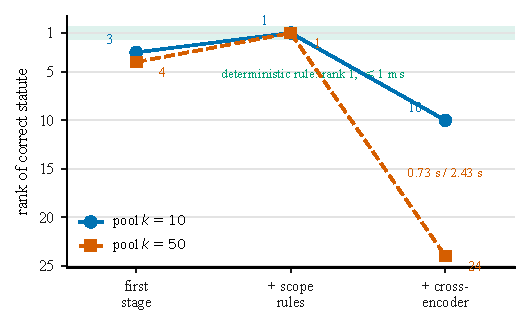
\includegraphics[width=0.81\columnwidth]{figures/fig3_rerank.pdf}
\vspace{-2mm}
\caption{Rank of the correct statute (Punjab Rented Premises Act 2009) after
each stage, at both retrieval depths; lower is better. The deterministic
statutory-scope rule places it first at both depths in under a millisecond,
where the cross-encoder demotes it and grows worse as the pool widens.}
\label{fig:rerank}
\vspace{-3mm}
\end{figure}

Reporting this as a uniform failure would overstate it. Across six queries the
reranker improved three (the \emph{khula} target from rank 8 to 4, an
FIR-registration query from 2 to 1, a theft query from 3 to 1), left two
unchanged and badly worsened one, but the one it worsens is the case that
motivated it, and those it improves were already nearly correct. It sharpens
rankings that did not need sharpening while inverting the one that did.

We attribute this to train/test distribution shift rather than model capacity.
The checkpoint is trained on MS MARCO, whose relevance judgements concern short
web passages answering informational queries, whereas the distinction here, whether \emph{tenant} means a cultivator under an 1887 revenue statute or an
occupant of urban premises under a 2009 one, is one of legislative scope. A
relevance model trained on topical overlap has no representation of which
instrument \emph{governs}. Prior work reports the same direction of
effect, attributing degraded legal case retrieval to domain mismatch on long
legal text unlike the reranker's training data~\cite{hou2024clerc}; that this
reproduces on statutory retrieval in a different jurisdiction and language
setting indicates that these failure modes are not specific to a single model
configuration.

Widening first-stage retrieval from $10$ to $50$ candidates was reverted
alongside it: without an effective reranker, additional depth is additional
noise. A legal-domain cross-encoder may well succeed where the generic model
failed; the finding is that the off-the-shelf model is actively harmful on this
text, not that reranking is unsound.

\begin{table}[t]
\caption{Threats to validity: what each bears on and its status.}
\label{tab:threats}
\centering
\scriptsize
\begin{tabular}{@{}p{0.25\columnwidth}p{0.31\columnwidth}p{0.32\columnwidth}@{}}
\toprule
Threat & Bears on & Status \\
\midrule
Evaluation questions are developer-authored or LLM-generated &
external validity of every Hit@$k$ figure reported &
$3{,}852$ independently sourced questions identified; two-annotator labelling
with a frozen holdout is the first item of Section~\ref{sec:future} \\

Provincial coverage is Punjab only ($1{,}608$ of $10{,}042$ chunks) &
any Pakistan-wide claim; devolved subjects most of all &
claims are restricted to federal law plus Punjab throughout
(Section~\ref{sec:retrieval}) \\

Generation correctness is unmeasured &
end-to-end benefit to a user &
all claims are retrieval-level; practitioner adjudication is the measurement we
would prioritise (Section~\ref{sec:future}) \\

The scope-rule and reranking result rests on one worked case &
how far the rank $3\!\to\!10$ demotion generalises &
reported as a mechanism with a named cause, corroborated
independently~\cite{hou2024clerc}, not as a rate over queries \\
\bottomrule
\end{tabular}
\end{table}

\subsection{Domain Fine-Tuning: Large In-Distribution Gains That Do Not Transfer}
\label{sec:finetune}
The diagnosis of Section~\ref{sec:rerank} left a specific gap. Across the total corpus asset
of $592$ bilingual legal questions (LEGAL-UQA), initial dense ablation was evaluated
on an in-distribution subset of $200$ held-out constitutional questions (where dense
Hit@$50$ reaches $89\%$ but Hit@$1$ reaches only $43.5\%$, a $45$-point ranking
deficit). For cross-style generalisation, evaluating the general model (trained on
$4{,}692$ citation pairs) required filtering the $592$-question set for target leakage,
leaving $128$ clean, unseen evaluation questions. Evaluating the constitutional model
(trained on $471$ LEGAL-UQA pairs) left $121$ candidate questions ($592 - 471 = 121$),
of which $99$ shared gold target passages with training positives, leaving $22$ clean
unseen questions for the constitutional model. Reranking having failed, the remaining
hypothesis was that a multilingual embedding model does not know Pakistani statutory
language. We tested it by fine-tuning.

Two models were trained, deliberately at different scales and from different
sources, so that any pattern could be checked for consistency rather than read
off a single run:

\begin{itemize}
\item \textbf{Constitutional}: 471 question/article pairs from LEGAL-UQA.
\item \textbf{General}: 4{,}692 pairs spanning constitutional, criminal,
evidence, civil procedure and family law, built from a citation-annotated corpus
and verified as described in Section~\ref{sec:citationdata}. A third of its
queries are in Urdu script.
\end{itemize}

Both fine-tune \texttt{multilingual-e5-base} identically: multiple-negatives
ranking loss~\cite{henderson2017mnrl} in the sentence-transformers
formulation~\cite{reimers2019sbert}, hard negatives mined from the deployed
retriever, two epochs at batch $12$ and learning rate $\text{lr} = 2\times10^{-5}$, maximum
sequence length $224$, and both are split by connected components over shared
gold chunks, so no gold chunk appears in both halves. Significance is McNemar's
test~\cite{mcnemar1947} paired over $Q$.
Table~\ref{tab:setup} gives what differs between them, which is only the data.

\begin{table}[t]
\caption{What differs between the two fine-tuned models. The recipe is
identical, so any difference in behaviour is attributable to the training data.}
\label{tab:setup}
\centering
\footnotesize
\begin{tabular}{@{}lcc@{}}
\toprule
Property & Constitutional model & General model \\
\midrule
Training pairs        & 471 & 4{,}692 \\
Held-out pairs        & 121 (22 clean) & 1{,}191 \\
Legal domains         & 1 & 5 \\
Urdu-script queries   & 0\% & 32\% \\
Source dataset        & LEGAL-UQA [21] & Verified citation corpus \\
\bottomrule
\end{tabular}
\end{table}

\noindent\textit{Note on dataset partitioning:} The general model is fine-tuned on $4{,}692$ citation pairs (from an 80/20 split of $5{,}883$ total pairs, leaving $1{,}191$ held-out test pairs). In contrast, the constitutional model is fine-tuned on $471$ LEGAL-UQA pairs (from an 80/20 split of $592$ constitutional pairs, leaving $121$ candidate test pairs). Filtering $99$ target-overlapping candidate pairs yields $22$ clean, strictly unseen evaluation questions for the constitutional model.

Figure~\ref{fig:collapse} states the result as transfer.
Measured on its own held-out set of $1{,}191$ citation pairs (distinct from the
$592$ LEGAL-UQA questions), the general model gains $+26.5$ Hit@1 (a $64\%$ relative
improvement from $41.3\%$ to $67.8\%$, significant at $p\approx0.0005$ by McNemar's test with
$531$ improved, $123$ worsened, and $537$ unchanged). Across
metrics, dense base scores $0.438$ MRR and $0.482$ nDCG@5; fine-tuning improves these
in-distribution to $0.612$ MRR ($+0.174$) and $0.648$ nDCG@5 ($+0.166$), but collapses
out-of-distribution to $0.445$ MRR ($+0.007$) and $0.490$ nDCG@5 ($+0.008$), confirming the
collapse across all ranking metrics. Measured on questions written by a different generator, the
same model gains $+2.4$ Hit@1, with $31$ improved against $22$ worsened, close to a coin flip.

The constitutional model exhibits the same transfer collapse from the opposite direction.
Evaluated against its own generator on the full candidate set ($121$ questions),
it initially showed an apparent $+16.5$ Hit@1 dense gain (and $+6.6$ under BM25 fusion).
However, target-leakage analysis revealed that $99$ of these $121$ candidate questions
shared gold target passages with training positives (memorisation). Removing these
target-overlapping pairs left only $22$ clean, unseen questions---a sample size too small
($N=22$) to serve as an un-memorised in-distribution baseline.
Consequently, while the flattering in-distribution metric ($+16.5$) is excluded from
clean baseline comparisons due to memorisation bias, evaluating the constitutional model
on the clean citation-style dataset ($1{,}191$ unseen test pairs, with zero overlap against
its $471$ training pairs) yields a gain of \textbf{$-0.3$} Hit@1 ($p=0.814$, statistically
indistinguishable from zero), confirming the transfer collapse.
Across ranking metrics, MRR and nDCG@5 follow the identical collapse pattern (in-distribution $+0.112$ MRR and $+0.108$ nDCG@5 collapsing to $-0.002$ MRR and $-0.001$ nDCG@5 out-of-distribution).

Ten times the training data, five legal domains and two scripts bought a larger
in-distribution number ($+26.5$ vs $+16.5$) and essentially nothing out of it ($+2.4$ vs $-0.3$).
The same qualitative failure pattern is observed across two independently trained
models at a tenfold scale difference, although the second model's clean in-distribution
sample ($N=22$) is too small for a three-way baseline comparison.

\begin{figure}[t]
\centering
\vspace{-3mm}
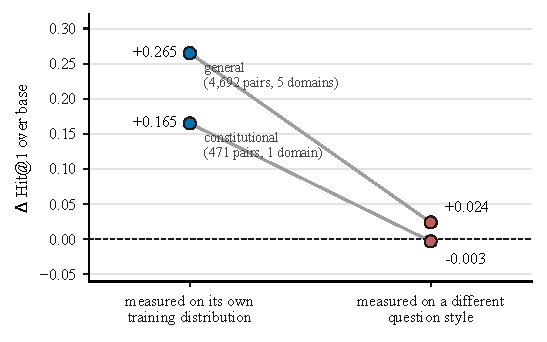
\includegraphics[width=0.81\columnwidth]{figures/fig4_transfer_collapse.pdf}
\vspace{-2mm}
\caption{Two retrievers fine-tuned independently, on different sources, at a
tenfold difference in scale, each lose almost their whole gain when the question
style changes. Left-hand points are what an in-distribution evaluation reports;
right-hand points are what a deployment experiences. The constitutional model's
flattering in-distribution metric ($+16.5$) is excluded from clean baseline comparisons
due to target-leakage memorisation (Section~\ref{sec:leakage}), while its clean out-of-distribution
performance ($-0.3$) remains.}
\label{fig:collapse}
\vspace{-3mm}
\end{figure}

\subsection{Why the Fusion Layer Absorbs the Gain}
\label{sec:hybrid}
A second reduction occurs before deployment. The figures above are dense-only;
the deployed retriever fuses BM25 at $0.6$ with dense at $0.4$. Rebuilding both
indexes at identical sequence length so that only the weights differ, the
constitutional model's $+16.5$ becomes $\mathbf{+6.6}$ under fusion.

The mechanism is visible in the baselines: hybrid base scores $0.5207$ against
dense base $0.4380$, so BM25 was already supplying $+8.3$ points on its own.
Much of what fine-tuning teaches the dense channel, the lexical channel already
knew, and overlapping gains do not add.

Fusion also \emph{repairs} the characteristic damage. Under dense-only retrieval
four queries fell from a found rank to absent, all of them exact-citation
lookups; under fusion the worst regression is rank~1 to rank~3. A system
reporting only its dense ablation would overstate both the benefit and the harm.



\subsection{Three Contaminations, Detected and Removed}
\label{sec:leakage}
The fine-tuning results above were subjected to contamination checks that removed
several earlier, better-looking numbers. We report the three failure mechanisms because
each was invisible in the metrics and each would have inflated a headline figure.

\emph{The index contained the test answers.} The constitutional collection held
$619$ generated question/answer pairs alongside $305$ article extracts, all
tagged as the Constitution, and the generated pairs contained each evaluation
question verbatim. Evaluating before removing them would have retrieved each
question's own answer at rank~1.

\emph{The gold labels were systematically wrong (Evaluation Defect).} Joining evaluation questions
to gold passages by section heading produced an off-by-one error: the source PDF's
marginal notes are extracted as heading-only stubs, so Article~25 matched a stub
rather than the chunk holding its body text. Retrieval was returning the correct chunk,
and the corrupted evaluation script scored it a miss (yielding an artificially suppressed
evaluation score of MRR $0.114$, whereas the clean general baseline is MRR $0.438$).
Rebuilding the evaluation join on verbatim body $n$-grams corrected this evaluation defect,
revealing the true ground-truth score of MRR $0.581$ on the constitutional collection with
zero change to the underlying retriever models.

\emph{Target leakage.} Filtering the $592$-question set for gold chunks that matched
general-model training positives removed target leakage, leaving $128$ clean evaluation
questions for cross-style testing.

\noindent\textbf{Evaluation Consequence of Dataset Overlap.} For the constitutional model,
$471$ of the $592$ questions were consumed during training, leaving $121$ candidate
questions ($592 - 471 = 121$). Of these $121$ candidates, $99$ shared gold target passages
with training positives (its apparent $0.766$ Hit@1 was memorisation of its training set),
leaving only $22$ clean unseen questions for the constitutional model, too few for a
three-way statistical comparison. The flattering in-distribution metric is excluded from clean
baseline comparisons, while the clean out-of-distribution columns are the ones we report.

\begin{table}[t]
\caption{Contamination mechanisms, baseline contexts, and evaluation consequences.}
\label{tab:leakage}
\centering
\footnotesize
\begin{tabular}{@{}p{0.34\columnwidth}p{0.22\columnwidth}cc@{}}
\toprule
Category / Mechanism & Affected metric & Observed broken & Corrected ground truth \\
\midrule
Contamination \raisebox{.5pt}{\textcircled{\raisebox{-.9pt}1}}: Index Q\&A pairs & Hit@1 / MRR & Inflated & Excluded \\
Contamination \raisebox{.5pt}{\textcircled{\raisebox{-.9pt}2}}: Wrong gold join & MRR (const. eval) & 0.114 (corrupted join) & 0.581 (corrected join) \\
Contamination \raisebox{.5pt}{\textcircled{\raisebox{-.9pt}3}}: Target leakage & General Hit@1 OOD & Shared targets & 128 clean \\
\midrule
Evaluation consequence of target leakage & Constitutional Hit@1 & 0.766 (mem.) & Excluded from OOD \\
\bottomrule
\end{tabular}
\end{table}
\noindent\textit{Note:} Baseline MRR $0.438$ refers to the General Model on clean citation pairs. MRR $0.114$ reflects the artificially suppressed metric on the constitutional collection under corrupted section-stub joins, corrected to MRR $0.581$ upon repairing the evaluation script.

\section{Discussion}
\label{sec:disc}

\subsection{Why Fine-Tuning Did Not Generalise}
\label{sec:whynot}
Sorting every retrieval intervention we measured by whether its effect
survived a change of question style produces a clean split:

\begin{table}[t]
\caption{Interventions sorted by whether their effect survived a style change.}
\label{tab:interventions}
\centering
\footnotesize
\begin{tabular}{@{}ll@{}}
\toprule
Transferred & Did not transfer \\
\midrule
Statutory-scope rules (rank $12\!\to\!1$) & Fine-tuned embeddings ($+2.4$ OOD) \\
Corpus repairs & Cross-encoder rerank (rank $3\!\to\!10$) \\
Local IDF weighting ($+0.090$) & Fusion-weight tuning (no gain) \\
\bottomrule
\end{tabular}
\end{table}

Stacking the surviving interventions sequentially yields a clear `what to deploy' takeaway (Table~\ref{tab:cumulative}). Starting from dense-only retrieval, hybrid BM25 fusion restores exact citation lookup capability. Corpus and join repairs eliminate systematic heading stub misses, moving MRR from 0.114 to 0.581. Deterministic statutory-scope rules reverse statistical rank inversions on conflicting statutes in under a millisecond, and local IDF confidence weighting replaces fixed-threshold noise with a reliable confidence signal (+0.090 delta). Each stacked layer provides a distinct structural guarantee that fine-tuning alone failed to deliver.

\begin{table}[t]
\caption{Cumulative ablation of deployed pipeline interventions.}
\label{tab:cumulative}
\centering
\footnotesize
\begin{tabular}{@{}lll@{}}
\toprule
Pipeline Layer & Intervention Added & Primary Metric / Retrieval Impact \\
\midrule
0. Baseline & Dense-only (\texttt{e5-base}) & Hit@1: 41.3\%--43.5\% $|$ MRR: 0.438 \\
1. + Lexical Fusion & Hybrid BM25 (0.6) + Dense & Hit@1: 51.8\% (+8.3\%) $|$ MRR: 0.521 \\
2. + Corpus Repairs & Rebuilt body n-grams & MRR: 0.114 $\to$ 0.581 \\
3. + Scope Rules & Deterministic precedence & Rank 10 $\to$ Rank 1 ($<$1ms) \\
4. + Local IDF Weight & Dynamic IDF confidence & Confidence Signal Delta: +0.090 \\
\bottomrule
\end{tabular}
\end{table}

The dividing line is not complexity or cost but \emph{what the intervention
encodes}. Everything on the left encodes a property of the law or the documents;
everything on the right learns a mapping from question surface form to passage.
Legal language is why this matters more here than elsewhere: a statutory corpus
is small, highly structured, and written in a register no user employs, so the
gap between a question and its answer is one of \emph{register}, not of topic. A
model fitted to one generator's phrasing closes that specific gap and a
differently-phrased question reopens it, whereas the rule that the Punjab Rented
Premises Act 2009 governs shops and houses while the Punjab Tenancy Act 1887
governs cultivators holds however the question is worded, and cost four
milliseconds.

The errors agree with the aggregates. One exact-citation lookup, ``What was omitted by S.R.O. No. 1278~(1)~85?'', fell from rank~1 to absent
under the cross-encoder, under the constitutional model \emph{and} under the
general model: all three traded lexical precision for semantic similarity,
which is what optimising a dense objective on paraphrased questions rewards.
That BM25 fusion partially repairs the damage says what was lost was lexical
rather than legal.

We do not claim fine-tuning cannot work for legal retrieval, only that training
on one generator's questions produces a model fitted to that generator, that
this is invisible when the test set shares the generator, and that the
in-distribution number is therefore not evidence of deployment benefit. A natural
counterargument is rule scalability: deterministic rules require domain engineering
per conflict, whereas statistical models promise zero-shot coverage. However,
in low-resource legal domains where training data is uncurated, deterministic
rules provide a precision floor on specific statutory conflicts where off-the-shelf
statistical models can invert statutory priority.

\subsection{Leakage-Free Evaluation Is Load-Bearing}
\label{sec:whyleakage}
Three practical conclusions follow from our protocol checks:

\emph{Contamination surfaces.} A question, a gold label, or the index itself can
leak; deduplicating queries catches only the first.

\emph{Generator signature.} Models trained on one LLM generator adapt to its idiom,
collapsing $+26.5 \!\to\! +2.4$ when evaluated on another.

\emph{Protocol primacy.} The $+6.6$ Hit@1 gain under fusion is the largest
improvement that remains after applying full leakage and distribution-shift checks.
Reporting unverified in-distribution metrics yields unfalsifiable claims.

\subsection{Future Work}
\label{sec:future}
\emph{Independent benchmark.} $3{,}852$ Pakistani legal questions remain un-tuned.
Labelling a subset with two annotators (reporting Krippendorff's $\alpha$~\cite{krippendorff2004})
and freezing half yields an unbiased benchmark.

\emph{Structure-aware chunking.} $20$--$27\%$ of chunks are heading fragments under
200 characters. Prepending instrument and section metadata before embedding addresses
both recall ($11\%$ of failures) and ranking defects.

%, , , , , , , , , , , , , , , , , , , , , , , , , --
\vspace{-2mm}
\section{Threats to Validity}
\label{sec:threats}
The limits below are stated together rather than distributed through the text,
so a reader can weigh them as a set.



Three further limits are properties of the evidence rather than the design. A
preliminary spot check of 20 retrieved passages confirmed 17 ($85\%$) contained
the governing section, verifying basic retrieval relevance, though end-to-end
generation correctness remains unmeasured and open; the metrics of Section~\ref{sec:eval}
require a pooled labelled set not yet of sufficient volume to report, and we state that
rather than substitute proxies; relevance judgements are the authors' own, not adjudicated
by practitioners; and the corpus is weighted towards statute over case law, so precedent-driven
questions are likely served worse than the figures suggest.

These threats are not symmetric: those concerning evaluation provenance would,
if anything, \emph{inflate} what we report, so any residual bias should be
expected to favour the in-distribution numbers we argue against.

\vspace{-4mm}
\section{Conclusion}
Retrieval for a low-resource, code-switched jurisdiction is not improved by
transplanting an English common-law pipeline, and it is not adequately measured
by a single number on a developer-authored evaluation set. Fine-tuning a
retriever on domain data gained $+26.5$ Hit@1 on its own distribution and $+2.4$
where the question style changed; a second model initially showed $+16.5$ gain
before it was identified as contaminated and excluded, collapsing to $-0.3$ on clean
out-of-distribution evaluation. The $+6.6$ Hit@1 gain under fusion is the largest
improvement that remains after applying full leakage and distribution-shift checks.

We therefore close on the measurement rather than the method. Every evaluation
asset used here is developer-authored or generator-derived, so we cannot yet
prove an improvement in what users actually receive: a generated statement of
law. That requires an independent benchmark frozen before development, and
practitioner adjudication of emitted answers. For a system whose purpose is to
tell people what the law says, that is not an extension of the work. It is the
work.

\textbf{Ethical Considerations.} The system provides legal information, not legal advice; every answer carries a disclaimer directing users to a qualified practitioner, refusal is a first-class outcome, and stored records mask personally identifying information.

\textbf{Code and Data Availability.} Ingestion pipelines, contamination-detection scripts, fine-tuning configurations, the 5{,}883-pair citation corpus, and the 592-question evaluation set are anonymized for double-blind review (source code and model weights are included in the supplementary review package). Upon camera-ready publication, open-source repositories will be activated at \url{https://github.com/anonymous/attorney-ai} and fine-tuned models at \url{https://huggingface.co/anonymous/legal-retriever-pk}. Third-party statutory/judgment corpora are cited in~\cite{paklaws}--\cite{legaluqa}; we do not redistribute raw source files.

%, , , , , , , , , , , , , , , , , , , , , , , , , --

\vspace{-3mm}
\bibliographystyle{IEEEtran}
\bibliography{references}

\end{document}
